\documentclass[12pt, A4]{article}\usepackage[]{graphicx}\usepackage[]{color}
%% maxwidth is the original width if it is less than linewidth
%% otherwise use linewidth (to make sure the graphics do not exceed the margin)
\makeatletter
\def\maxwidth{ %
  \ifdim\Gin@nat@width>\linewidth
    \linewidth
  \else
    \Gin@nat@width
  \fi
}
\makeatother

\definecolor{fgcolor}{rgb}{0.345, 0.345, 0.345}
\newcommand{\hlnum}[1]{\textcolor[rgb]{0.686,0.059,0.569}{#1}}%
\newcommand{\hlstr}[1]{\textcolor[rgb]{0.192,0.494,0.8}{#1}}%
\newcommand{\hlcom}[1]{\textcolor[rgb]{0.678,0.584,0.686}{\textit{#1}}}%
\newcommand{\hlopt}[1]{\textcolor[rgb]{0,0,0}{#1}}%
\newcommand{\hlstd}[1]{\textcolor[rgb]{0.345,0.345,0.345}{#1}}%
\newcommand{\hlkwa}[1]{\textcolor[rgb]{0.161,0.373,0.58}{\textbf{#1}}}%
\newcommand{\hlkwb}[1]{\textcolor[rgb]{0.69,0.353,0.396}{#1}}%
\newcommand{\hlkwc}[1]{\textcolor[rgb]{0.333,0.667,0.333}{#1}}%
\newcommand{\hlkwd}[1]{\textcolor[rgb]{0.737,0.353,0.396}{\textbf{#1}}}%
\let\hlipl\hlkwb

\usepackage{framed}
\makeatletter
\newenvironment{kframe}{%
 \def\at@end@of@kframe{}%
 \ifinner\ifhmode%
  \def\at@end@of@kframe{\end{minipage}}%
  \begin{minipage}{\columnwidth}%
 \fi\fi%
 \def\FrameCommand##1{\hskip\@totalleftmargin \hskip-\fboxsep
 \colorbox{shadecolor}{##1}\hskip-\fboxsep
     % There is no \\@totalrightmargin, so:
     \hskip-\linewidth \hskip-\@totalleftmargin \hskip\columnwidth}%
 \MakeFramed {\advance\hsize-\width
   \@totalleftmargin\z@ \linewidth\hsize
   \@setminipage}}%
 {\par\unskip\endMakeFramed%
 \at@end@of@kframe}
\makeatother

\definecolor{shadecolor}{rgb}{.97, .97, .97}
\definecolor{messagecolor}{rgb}{0, 0, 0}
\definecolor{warningcolor}{rgb}{1, 0, 1}
\definecolor{errorcolor}{rgb}{1, 0, 0}
\newenvironment{knitrout}{}{} % an empty environment to be redefined in TeX

\usepackage{alltt}
%\usepackage[brazil]{babel}
\usepackage{graphicx}
\usepackage[utf8]{inputenc}
\usepackage[T1]{fontenc}
\usepackage{url}
\usepackage{natbib}
\usepackage{amsmath}
\bibliographystyle{rusnat}
\usepackage{framed, color}
\usepackage{xspace}
\definecolor{shadecolor}{rgb}{0.9, 0.9, 0.9}
\newcommand{\R}{\textnormal{\sffamily\bfseries R}\xspace}
\newcommand{\code}[1]{\texttt{#1}}


\title{Estimates of total tree richness in Amazon - Summary}
\author{Han Ter Steege, Paulo Inácio Prado, Renato Lima, ATDN}
\IfFileExists{upquote.sty}{\usepackage{upquote}}{}
\begin{document}

\maketitle




\section{Data preparation}

\begin{knitrout}
\definecolor{shadecolor}{rgb}{0.969, 0.969, 0.969}\color{fgcolor}\begin{kframe}
\begin{alltt}
\hlstd{Dec2018} \hlkwb{<-} \hlkwd{read.csv2}\hlstd{(}\hlstr{"Populations_2018_V2b.csv"}\hlstd{,} \hlkwc{as.is}\hlstd{=}\hlnum{TRUE}\hlstd{)}
\hlstd{N.ind} \hlkwb{<-} \hlstd{Dec2018}\hlopt{$}\hlstd{N.ind}
\hlstd{Sobs} \hlkwb{<-} \hlkwd{length}\hlstd{(N.ind)}
\hlcom{## Total number of trees (average density x area)}
\hlstd{Tot.t} \hlkwb{<-} \hlnum{567}\hlopt{*}\hlnum{5.5e8}
\hlcom{## Proportion of total trees in the sample}
\hlstd{p1} \hlkwb{<-} \hlkwd{sum}\hlstd{(Dec2018}\hlopt{$}\hlstd{N.ind)}\hlopt{/}\hlstd{Tot.t}
\hlcom{## Total number of plots}
\hlstd{N.plots} \hlkwb{<-} \hlnum{1945}
\hlcom{## Total area hectares}
\hlstd{Tot.A} \hlkwb{<-} \hlnum{5.79e8}
\hlcom{## Sampled area ha}
\hlstd{Samp.A} \hlkwb{<-} \hlnum{2.048e3}
\end{alltt}
\end{kframe}
\end{knitrout}

\section{Estimates from the plots sample}

\subsection*{Poisson lognormal}

Seems to overestimate the abundance of the most abundant species (see qq-plots)
 
\begin{knitrout}
\definecolor{shadecolor}{rgb}{0.969, 0.969, 0.969}\color{fgcolor}\begin{kframe}
\begin{alltt}
\hlstd{pln} \hlkwb{<-} \hlkwd{fitpoilog}\hlstd{(N.ind)}
\hlkwd{par}\hlstd{(}\hlkwc{mfrow}\hlstd{=}\hlkwd{c}\hlstd{(}\hlnum{2}\hlstd{,}\hlnum{2}\hlstd{))}
\hlkwd{plot}\hlstd{(pln)}
\hlkwd{par}\hlstd{(}\hlkwc{mfrow}\hlstd{=}\hlkwd{c}\hlstd{(}\hlnum{1}\hlstd{,}\hlnum{1}\hlstd{))}
\end{alltt}
\end{kframe}

{\centering 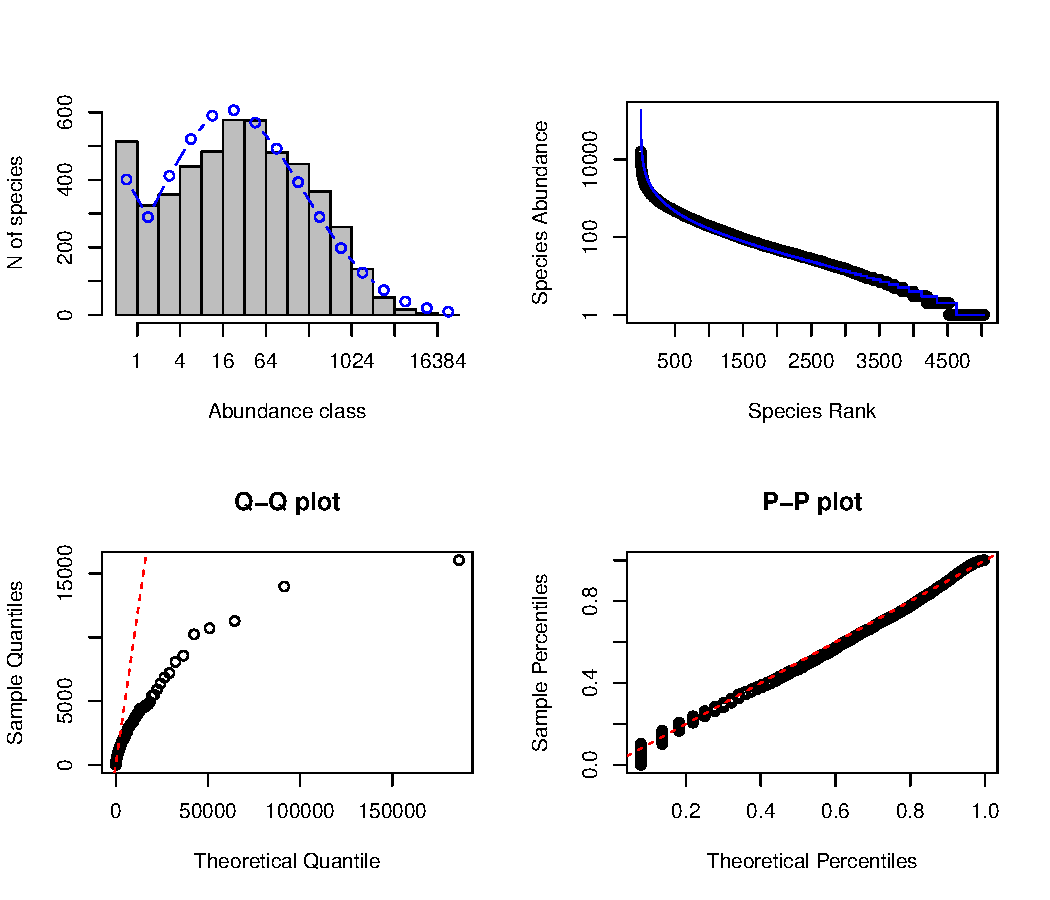
\includegraphics[width=\maxwidth]{figure/fit_pln-1} 

}



\end{knitrout}


\subsubsection*{Estimating species richness from PLN}

The fitted PLN allows to estimate the probability value assigned to species that
had zero abundance in the sample:

\begin{knitrout}
\definecolor{shadecolor}{rgb}{0.969, 0.969, 0.969}\color{fgcolor}\begin{kframe}
\begin{alltt}
\hlstd{pln.cf} \hlkwb{<-} \hlkwd{coef}\hlstd{(pln)}
\hlstd{(pln.d0} \hlkwb{<-} \hlkwd{dpoilog}\hlstd{(}\hlnum{0}\hlstd{,} \hlkwc{mu} \hlstd{= pln.cf[}\hlnum{1}\hlstd{],} \hlkwc{sig}\hlstd{=pln.cf[}\hlnum{2}\hlstd{]))}
\end{alltt}
\begin{verbatim}
## [1] 0.11
\end{verbatim}
\end{kframe}
\end{knitrout}

That is, an estimate that the recorded species are 89\%
of the total number of species.
This gives an estimate of 5652 species.


\subsection*{Log-series}

Log-series seems to overestimate the number of singletons
and to underestimate the abundance of species with intermediary abundances
(between 16 and 64 individuals, see octave plot). Also, the qq-plot shows that
the model underestimates the larger abundances.

 
\begin{knitrout}
\definecolor{shadecolor}{rgb}{0.969, 0.969, 0.969}\color{fgcolor}\begin{kframe}
\begin{alltt}
\hlstd{y.ls} \hlkwb{<-} \hlkwd{fitls}\hlstd{(N.ind)}
\hlkwd{par}\hlstd{(}\hlkwc{mfrow}\hlstd{=}\hlkwd{c}\hlstd{(}\hlnum{2}\hlstd{,}\hlnum{2}\hlstd{))}
\hlkwd{plot}\hlstd{(y.ls)}
\hlkwd{par}\hlstd{(}\hlkwc{mfrow}\hlstd{=}\hlkwd{c}\hlstd{(}\hlnum{1}\hlstd{,}\hlnum{1}\hlstd{))}
\end{alltt}
\end{kframe}

{\centering 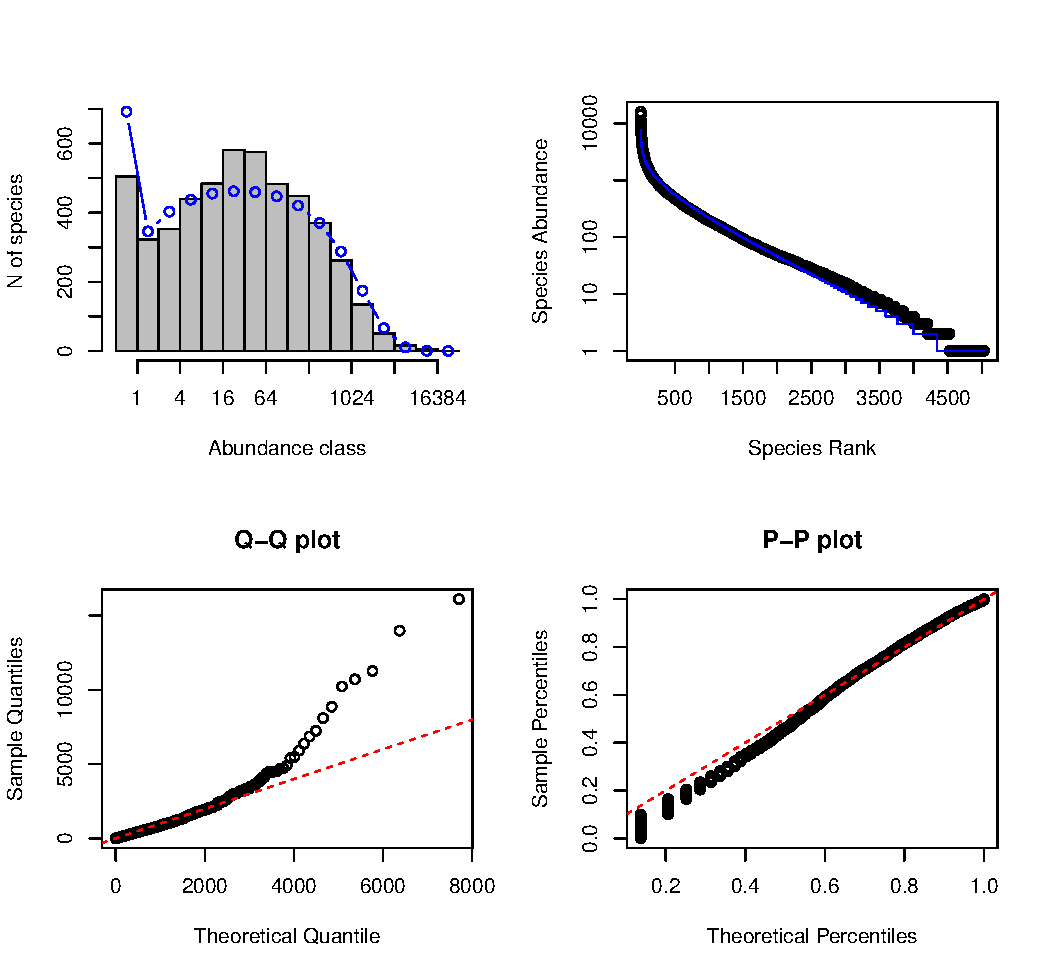
\includegraphics[width=\maxwidth]{figure/fit_ls-1} 

}



\end{knitrout}

\subsubsection*{Estimate of species richness from LS}

From the value of $\alpha$ estimated from the sample of plots:
 
\begin{knitrout}
\definecolor{shadecolor}{rgb}{0.969, 0.969, 0.969}\color{fgcolor}\begin{kframe}
\begin{alltt}
\hlstd{alpha} \hlkwb{<-} \hlkwd{coef}\hlstd{(y.ls)[[}\hlnum{2}\hlstd{]]}
\hlstd{(S.ls} \hlkwb{<-} \hlstd{alpha}\hlopt{*}\hlkwd{log}\hlstd{(}\hlnum{1} \hlopt{+} \hlstd{Tot.t}\hlopt{/}\hlstd{alpha))}
\end{alltt}
\begin{verbatim}
## [1] 13802
\end{verbatim}
\end{kframe}
\end{knitrout}

And here is the confidence interval for Fisher's $\alpha$ and the
interval for estimated total richness from these values

\begin{knitrout}
\definecolor{shadecolor}{rgb}{0.969, 0.969, 0.969}\color{fgcolor}\begin{kframe}
\begin{alltt}
\hlstd{(ls.ci} \hlkwb{<-} \hlkwd{confint}\hlstd{(y.ls))}
\end{alltt}
\begin{verbatim}
##  2.5 % 97.5 % 
##    638    750
\end{verbatim}
\begin{alltt}
\hlcom{## Estimated species richness for lower bound of alpha's IC}
\hlstd{ls.ci[}\hlnum{1}\hlstd{]}\hlopt{*}\hlkwd{log}\hlstd{(}\hlnum{1} \hlopt{+} \hlstd{Tot.t}\hlopt{/}\hlstd{ls.ci[}\hlnum{1}\hlstd{])}
\end{alltt}
\begin{verbatim}
## 2.5 % 
## 12774
\end{verbatim}
\begin{alltt}
\hlstd{ls.ci[}\hlnum{2}\hlstd{]}\hlopt{*}\hlkwd{log}\hlstd{(}\hlnum{1} \hlopt{+} \hlstd{Tot.t}\hlopt{/}\hlstd{ls.ci[}\hlnum{2}\hlstd{])}
\end{alltt}
\begin{verbatim}
## 97.5 % 
##  14878
\end{verbatim}
\end{kframe}
\end{knitrout}

\subsection*{Zero-truncated Negative binomial}
\label{sec:negbin}

Here I use the method proposed by \citet{tovo2017}. The first step is
to fit a zero-truncated negative binomial (TNB) to the abundances in the sample.
I did that with the \emph{VGAM} package (as the authors did)
and also with the \emph{sads} package. 
The results were similar, and the fit looks identical to
those provided by the log-series (but has much lower AIC value, see below).
 
\begin{knitrout}
\definecolor{shadecolor}{rgb}{0.969, 0.969, 0.969}\color{fgcolor}\begin{kframe}
\begin{alltt}
\hlcom{## With VGAM}
\hlstd{y.nb} \hlkwb{<-} \hlkwd{vglm}\hlstd{(N.ind} \hlopt{~} \hlnum{1}\hlstd{, posnegbinomial)}
\hlcom{## With sads}
\hlstd{y.nb2} \hlkwb{<-} \hlkwd{fitnbinom}\hlstd{(N.ind,}
                   \hlkwc{start.value}\hlstd{=}\hlkwd{c}\hlstd{(}\hlkwc{size}\hlstd{=}\hlnum{0.3}\hlstd{,} \hlkwc{mu}\hlstd{=}\hlkwd{mean}\hlstd{(N.ind)))}
\hlcom{## Comparing: }
\hlkwd{exp}\hlstd{(}\hlkwd{coef}\hlstd{(y.nb))}
\end{alltt}
\begin{verbatim}
## (Intercept):1 (Intercept):2 
##   52.11347189    0.04344702
\end{verbatim}
\begin{alltt}
\hlkwd{coef}\hlstd{(y.nb2)}
\end{alltt}
\begin{verbatim}
##        size          mu 
##  0.04404989 52.74636711
\end{verbatim}
\end{kframe}
\end{knitrout}

\begin{knitrout}
\definecolor{shadecolor}{rgb}{0.969, 0.969, 0.969}\color{fgcolor}\begin{kframe}
\begin{alltt}
\hlkwd{par}\hlstd{(}\hlkwc{mfrow}\hlstd{=}\hlkwd{c}\hlstd{(}\hlnum{2}\hlstd{,}\hlnum{2}\hlstd{))}
\hlkwd{plot}\hlstd{(y.nb2)}
\hlkwd{par}\hlstd{(}\hlkwc{mfrow}\hlstd{=}\hlkwd{c}\hlstd{(}\hlnum{1}\hlstd{,}\hlnum{1}\hlstd{))}
\end{alltt}
\end{kframe}

{\centering 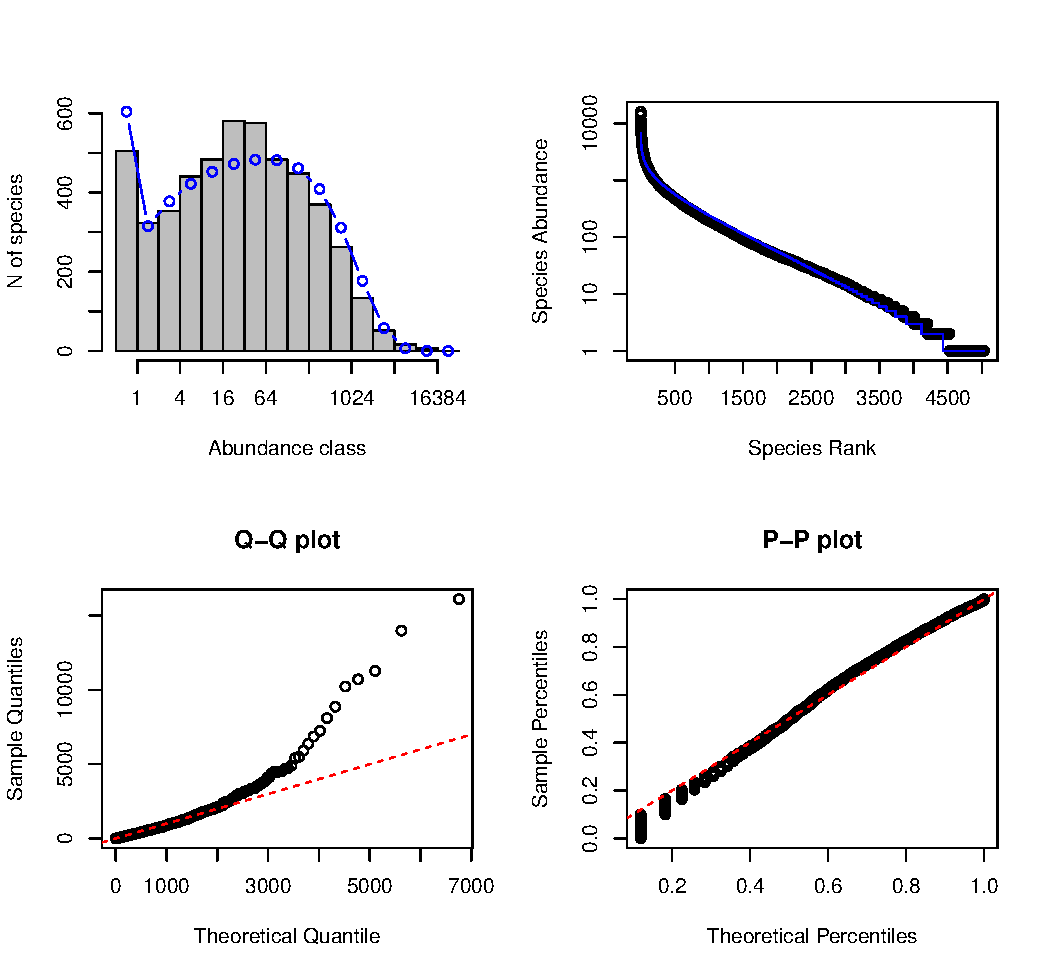
\includegraphics[width=\maxwidth]{figure/nb_plots-1} 

}



\end{knitrout}


\subsubsection*{Estimate of  species richness}

Following the recipe of \citet{tovo2017}:

 
\begin{knitrout}
\definecolor{shadecolor}{rgb}{0.969, 0.969, 0.969}\color{fgcolor}\begin{kframe}
\begin{alltt}
\hlstd{cf.nb} \hlkwb{<-} \hlkwd{coef}\hlstd{(y.nb2)}
\hlstd{csi.p} \hlkwb{<-} \hlkwd{unname}\hlstd{(cf.nb[}\hlnum{2}\hlstd{]}\hlopt{/}\hlstd{(}\hlkwd{sum}\hlstd{(cf.nb)))}
\hlstd{csi} \hlkwb{<-} \hlstd{csi.p}\hlopt{/}\hlstd{(p1}\hlopt{+}\hlstd{(}\hlnum{1}\hlopt{-}\hlstd{p1)}\hlopt{*}\hlstd{csi.p)}
\hlcom{## Estimated number of species }
\hlstd{S.nb} \hlkwb{<-} \hlstd{Sobs}\hlopt{*}\hlstd{(}\hlnum{1}\hlopt{-}\hlstd{(}\hlnum{1}\hlopt{-}\hlstd{csi)}\hlopt{^}\hlstd{cf.nb[}\hlnum{1}\hlstd{])} \hlopt{/} \hlstd{(}\hlnum{1}\hlopt{-}\hlstd{(}\hlnum{1}\hlopt{-}\hlstd{csi.p)}\hlopt{^}\hlstd{cf.nb[}\hlnum{1}\hlstd{])}
\hlstd{(S.nb} \hlkwb{<-} \hlkwd{unname}\hlstd{(S.nb))}
\end{alltt}
\begin{verbatim}
## [1] 10901
\end{verbatim}
\end{kframe}
\end{knitrout}

I did a simple function to automate the calculations and to return
the confidence intervals, based on the confidence intervals of the 
coefficients of the NB fit (see file \code{functions.R})

 
\begin{knitrout}
\definecolor{shadecolor}{rgb}{0.969, 0.969, 0.969}\color{fgcolor}\begin{kframe}
\begin{alltt}
\hlstd{(tovo.S} \hlkwb{<-} \hlkwd{tovo}\hlstd{(}\hlkwc{fit} \hlstd{= y.nb2,} \hlkwc{p} \hlstd{= p1,} \hlkwc{CI}\hlstd{=}\hlnum{TRUE}\hlstd{))}
\end{alltt}
\begin{verbatim}
## Estimated species richness: 10901 
##  95% CI: 10137 - 11868
## $S.est
## [1] 10901
## 
## $CIs
##         2.5 %  97.5 %
## size  2.8e-02 5.9e-02
## mu    3.6e+01 6.7e+01
## prob  2.5e-09 2.8e-09
## S.est 1.2e+04 1.0e+04
\end{verbatim}
\end{kframe}
\end{knitrout}


\subsection*{Model selection}

Among the three models, TNB
provides the best fit to the abundances in the sample:

 
\begin{knitrout}
\definecolor{shadecolor}{rgb}{0.969, 0.969, 0.969}\color{fgcolor}\begin{kframe}
\begin{alltt}
\hlkwd{AICtab}\hlstd{(pln, y.nb2, y.ls,} \hlkwc{base}\hlstd{=}\hlnum{TRUE}\hlstd{)}
\end{alltt}
\begin{verbatim}
##       AIC   dAIC  df
## y.nb2 54627     0 2 
## y.ls  54658    31 1 
## pln   54667    40 2
\end{verbatim}
\end{kframe}
\end{knitrout}

TNB overestimates the higher abundances, while the logseries
underestimates the lower abundances in the sample:

\begin{knitrout}
\definecolor{shadecolor}{rgb}{0.969, 0.969, 0.969}\color{fgcolor}

{\centering \includegraphics[width=\maxwidth]{figure/Comparing_LS_and_NB-1} 

}



\end{knitrout}

\section{Estimates based in the RAD of population sizes}

\subsection*{Linear extrapolation from the regional RAD}

Here I replicated the extrapolation method from the RAD of the
estimated abundances for the whole Amazonia first for the logseries projection:

\begin{knitrout}
\definecolor{shadecolor}{rgb}{0.969, 0.969, 0.969}\color{fgcolor}\begin{kframe}
\begin{alltt}
\hlstd{S.ulrich} \hlkwb{<-} \hlkwd{ulrich}\hlstd{(Dec2018}\hlopt{$}\hlstd{population)}
\hlstd{(S.r.ls} \hlkwb{<-} \hlstd{S.ulrich}\hlopt{$}\hlstd{S[}\hlnum{1}\hlstd{])}
\end{alltt}
\begin{verbatim}
## [1] 15279
\end{verbatim}
\end{kframe}
\end{knitrout}

Which are exactly the value reported in the manuscript (15279 species). 
Thus, from this estimate the value of Fisher's $\alpha$ for the whole Amazon is

\begin{knitrout}
\definecolor{shadecolor}{rgb}{0.969, 0.969, 0.969}\color{fgcolor}\begin{kframe}
\begin{alltt}
\hlstd{(alpha.r} \hlkwb{<-} \hlkwd{fishers.alpha}\hlstd{(}\hlkwc{N} \hlstd{= Tot.t,} \hlkwc{S} \hlstd{= S.r.ls))}
\end{alltt}
\begin{verbatim}
## [1] 771
\end{verbatim}
\end{kframe}
\end{knitrout}

And with this estimate of regional $\alpha$ we can build a RAD for the Amazon \citep{tersteege2013}.
I made a function to calculate the regional RAD which runs faster than the original code.
Using it we get the log-series RAD for the whole region (Amazon):

\begin{knitrout}
\definecolor{shadecolor}{rgb}{0.969, 0.969, 0.969}\color{fgcolor}\begin{kframe}
\begin{alltt}
\hlstd{reg.ls.rad} \hlkwb{<-} \hlkwd{ceiling}\hlstd{(}
    \hlkwd{rad.ls}\hlstd{(}\hlkwc{S} \hlstd{= S.r.ls,} \hlkwc{N} \hlstd{= Tot.t,} \hlkwc{alpha} \hlstd{= alpha.r)}\hlopt{$}\hlstd{y}
\hlstd{)}
\end{alltt}
\end{kframe}
\end{knitrout}

\subsubsection*{Lower limit of the linear extrapolation}

According to \citet{ulrich2005}, the estimate from the linear extrapolation of LS is an upper limit to the estimation of species. 
They propose that the same linear extrapolation assuming a log-normal is a lower-bound estimate.
Following their recipe (eq.2) such lower bound would be:

\begin{knitrout}
\definecolor{shadecolor}{rgb}{0.969, 0.969, 0.969}\color{fgcolor}\begin{kframe}
\begin{alltt}
\hlstd{(S.ulrich}\hlopt{$}\hlstd{S[}\hlnum{2}\hlstd{])}
\end{alltt}
\begin{verbatim}
## [1] 12785
\end{verbatim}
\end{kframe}
\end{knitrout}


\subsection*{Regional RAD from TNB}

The RAD of negative binomial was upscaled according to \citep{tovo2017} 
and gets to the number of species estimated by this method (section~\ref{sec:negbin}).
I did a function that returns this upscaled RAD pretty fast

\begin{knitrout}
\definecolor{shadecolor}{rgb}{0.969, 0.969, 0.969}\color{fgcolor}\begin{kframe}
\begin{alltt}
\hlstd{reg.nb.rad} \hlkwb{<-} \hlkwd{rad.posnegbin}\hlstd{(}\hlkwc{S} \hlstd{= S.nb,} \hlkwc{size} \hlstd{= cf.nb[}\hlnum{1}\hlstd{],}
                            \hlkwc{prob} \hlstd{=} \hlnum{1}\hlopt{-}\hlstd{csi)}\hlopt{$}\hlstd{y}
\end{alltt}
\end{kframe}
\end{knitrout}

Now we have the LS and TNB regional RADs 
I will plot them with the RAD of estimated population sizes, and also
with the upper-bound and lower-bound estimate of species
obtained above.


\begin{knitrout}
\definecolor{shadecolor}{rgb}{0.969, 0.969, 0.969}\color{fgcolor}

{\centering \includegraphics[width=\maxwidth]{figure/nbinom_rad-1} 

}



\end{knitrout}

The blue line is the RAD predicted by zero-truncated negative binomial upscaled to the total number of
trees in Amazonia. %Broken lines are approximated 95\% CIs. 
The red line is the upscaled log-series for the Amazon,
as sent by Hans ( file \code{script\_for\_Paulo.R} ). 
Black lines are the linear extrapolations for the 50\% 
central quantile of the estimated population sizes, for
the Log-series and log-normal model \citep{ulrich2005}.

The negative binomial has a power-bending factor that
results in a lower estimate of total richness, below to
the lower-limit of the linear extrapolations.

The next section has uses a Bayesian approach to identify
the regional RAD model and also the sampling model that 
best approximates the RAD of population sizes.

\section{Comparing population sizes predicted by LS and NB regional RADs}

\subsection*{Methods}

To check which RAD model would approximate better the total population sizes estimated
for the sampled species, we simulated samples from the Amazon RAD generated by the Log-series 
and Truncated Negative Binomial, with and without clumping. 
In both cases we assumed a random drawn of 1945 1-ha plots
from the Amazon RADs, where the number of individuals of each species
in each plot followed a Poisson (random sampling) or a Negative Binomial (clumped sampling)
distribution. 

The simulated population sizes where the total population sizes taken from
the regional RAD, only for those species that had been recorded 
in the simulated sample. 
The probability of each species be not included in a sample of $N$ plots is  $P(0)=(1-p)^N$.

Where $p$ is the probability of occurrence in each plot. 
Given the density of the species per plot $\mu$, 
for a Poisson sample 

\begin{equation}
  \label{eq:3}
  P(0) = e^{-\mu} 
\end{equation} 

and for a Negative Binomial sample

\begin{equation}
  \label{eq:2}
  P(0) = \left( \frac{k}{k+\mu} \right)^k 
\end{equation}

Where $k$ is the dispersion parameter of the negative binomial distribution.
%This coefficient adds extra variance compared to a Poisson sampling.
Thus we simulated occurrences of each species by sampling presence/absences
from a Bernoulli distribution with probability of occurrence $1-P(0)$.

\subsubsection*{Simulating clumping coefficients}

For simulations of clumped sampling, 
we allowed interspecific variation in clumping, 
by allowing a different value of the dispersion coefficient ($k$) for each species.
Hence, we had to define the value of $k$ for each species in the regional
RADs. We did that by (i) estimating the values of $k$ for the sampled species and
then (ii) by using the relationship between $k$ and $\mu$ to estimate the values of $k$
of each species.

To estimate the values of the aggregation coefficients
of the sampled species
we assumed that the number of plots that each species has been recorded follows
a binomial distribution with a probability of occurrence in each plot of $p=1-P(0)$,
with $P(0)$ from equation~\ref{eq:2}.
The parameter $k$ was then estimated by numerically maximizing the
log-likelihood function of the binomial distribution:

\begin{equation}
  \mathcal{L}(k | \mu, N, f_0) \ =  \ f_0 \ln (1-p) + (N - f_0) \ln p
\end{equation}

Where $N$ is the total number of plots, $f_0$ is 
the number of plots where the species was not recorded.
This log-likelihood function is conditioned to $\mu$, because this parameter was 
set to the observed density of each species in the sample.

Once we estimated a value of $k$ for each species recorded, 
we fit a linear regression of these values in function of the
observed species densities in the sample, in log scale.
The commands and model summary are:

\begin{knitrout}
\definecolor{shadecolor}{rgb}{0.969, 0.969, 0.969}\color{fgcolor}\begin{kframe}
\begin{alltt}
\hlcom{## estimating k parameter of a NB for each species }
\hlstd{Dec2018}\hlopt{$}\hlstd{dens.ha} \hlkwb{<-} \hlstd{Dec2018}\hlopt{$}\hlstd{N.ind}\hlopt{/}\hlstd{Samp.A}
\hlstd{Dec2018}\hlopt{$}\hlstd{k} \hlkwb{<-} \hlkwd{est.kv}\hlstd{(}\hlkwc{mu}\hlstd{=Dec2018}\hlopt{$}\hlstd{dens.ha,}
                  \hlkwc{nzeroes}\hlstd{=N.plots}\hlopt{-}\hlstd{Dec2018}\hlopt{$}\hlstd{N.plots,}
                  \hlkwc{Nplots}\hlstd{=N.plots)}
\hlstd{lm.k} \hlkwb{<-}\hlkwd{lm}\hlstd{(}\hlkwd{log}\hlstd{(k)}\hlopt{~}\hlkwd{log}\hlstd{(dens.ha),}
          \hlkwc{data}\hlstd{=Dec2018,} \hlkwc{subset}\hlstd{=k}\hlopt{<}\hlnum{1}\hlstd{)}
\hlcom{## Estimated regression standard error}
\hlstd{lm.k.sigma} \hlkwb{<-} \hlkwd{summary}\hlstd{(lm.k)}\hlopt{$}\hlstd{sigma}
\hlcom{## Model summary}
\hlkwd{summary}\hlstd{(lm.k)}
\end{alltt}
\begin{verbatim}
## 
## Call:
## lm(formula = log(k) ~ log(dens.ha), data = Dec2018, subset = k < 
##     1)
## 
## Residuals:
##     Min      1Q  Median      3Q     Max 
## -5.3939 -0.6564  0.1166  0.8321  5.1151 
## 
## Coefficients:
##              Estimate Std. Error t value Pr(>|t|)    
## (Intercept)  -3.09932    0.04412  -70.24   <2e-16 ***
## log(dens.ha)  0.59059    0.01065   55.45   <2e-16 ***
## ---
## Signif. codes:  0 '***' 0.001 '**' 0.01 '*' 0.05 '.' 0.1 ' ' 1
## 
## Residual standard error: 1.234 on 4196 degrees of freedom
## Multiple R-squared:  0.4229,	Adjusted R-squared:  0.4227 
## F-statistic:  3074 on 1 and 4196 DF,  p-value: < 2.2e-16
\end{verbatim}
\end{kframe}
\end{knitrout}

And a plot of with the regression line is

\begin{knitrout}
\definecolor{shadecolor}{rgb}{0.969, 0.969, 0.969}\color{fgcolor}

{\centering \includegraphics[width=\maxwidth]{figure/lok_k_x_log_density_plot-1} 

}



\end{knitrout}

We then used this regression model to set a value of $k$ for each species from
their abundances as predicted by the regional RAD. 
In each simulation we drawn a value of $\ln k$ for each species
in the Amazon RAD from a Normal distribution with the mean as
the predicted value from the linear regression above for the population
density of the species in the RAD. The standard deviation of these
Normal distributions was the standard error of the linear regression.

\subsubsection*{Fit to observed population sizes}
\label{sec:fit-observ-popul}

To check which model best describes the RAD of estimated population we
used an approximate Bayesian computation (ABC, \citet{csillery2010,csillery2012}). 
To do that I ran 
the simulations described above for each combination of RAD and sampling
for 6135 values of regional richness, drawn from a uniform
distribution between 10,000 and 20,000. In ABC this is the \emph{a priori}
distribution, which I set between the know number of species in Amazon and
twice it, which is higher the larger species estimate for Amazon I get.

The ABC method compares summary statistics from the simulations with those observed
in a dataset to assign (approximate) posterior probabilities to each competing model.
I used four statistics from the simulated population RADs: number of species, inverse of Simpson's index
(that is, Simpson's species equivalents), and mean an standard deviation of the log of abundances.

The observed values of the statistics are targets against the results of each simulations is compared with an standardized
Euclidean distance. The proportion of simulations of each model that are below a gives distance threshold estimates the
posterior probability of the model, and thus provides a model-selection criteria based on computational simulations.
A similar procedure is used to estimate the posterior distribution of the parameters of the simulation, which in this case
was only the total number of species in the regional RAD from which the simulated samples were drawn.

I used a rejection threshold of 0.025, which means that only the 2,5\% simulations that resulted in the smallest Euclidean
distances to the observed values of the summary statistics were kept to build posterior distributions.
The codes used to run ABC are in separated file (\code{abc.R}), as the simulations take some time to run.


\subsection*{Results}

ABC model selection, using a 5\% rejection threshold:

\begin{knitrout}
\definecolor{shadecolor}{rgb}{0.969, 0.969, 0.969}\color{fgcolor}\begin{kframe}
\begin{alltt}
\hlcom{## load simulation objects to be used by ABC}
\hlkwd{load}\hlstd{(}\hlstr{"abc_1000_to_2000_S.RData"}\hlstd{)}
\hlcom{## Target: observed number of species, Simpson's 1/D, }
\hlcom{## lmean, sdmean             }
\hlstd{target} \hlkwb{<-} \hlkwd{c}\hlstd{(Sobs,}
            \hlkwd{D}\hlstd{(Dec2018}\hlopt{$}\hlstd{population),}
            \hlkwd{mean}\hlstd{(}\hlkwd{log}\hlstd{(Dec2018}\hlopt{$}\hlstd{population)),}
            \hlkwd{sd}\hlstd{(}\hlkwd{log}\hlstd{(Dec2018}\hlopt{$}\hlstd{population)))}
\hlcom{## Model selection}
\hlstd{model.sel} \hlkwb{<-} \hlkwd{postpr}\hlstd{(}\hlkwc{target} \hlstd{= target,}
                    \hlkwc{index}\hlstd{=sim.ids,}
                    \hlkwc{sumstat} \hlstd{= all.sims,}
                    \hlkwc{tol}\hlstd{=}\hlnum{0.05}\hlstd{,} \hlkwc{method}\hlstd{=}\hlstr{"rejection"}\hlstd{,}
                    \hlkwc{corr}\hlstd{=}\hlnum{TRUE}\hlstd{)}
\hlstd{msel.s} \hlkwb{<-} \hlkwd{summary}\hlstd{(model.sel)}
\end{alltt}
\begin{verbatim}
## Call: 
## postpr(target = target, index = sim.ids, sumstat = all.sims, 
##     tol = 0.05, method = "rejection", corr = TRUE)
## Data:
##  postpr.out$values (898 posterior samples)
## Models a priori:
##  LSclump, LSrnd, NBclump, NBrnd
## Models a posteriori:
##  LSclump, LSrnd, NBclump, NBrnd
## 
## 
## Proportion of accepted simulations (rejection):
## LSclump   LSrnd NBclump   NBrnd 
##   0.996   0.004   0.000   0.000 
## 
## Bayes factors:
##         LSclump   LSrnd NBclump   NBrnd
## LSclump   1.000 223.500     Inf     Inf
## LSrnd     0.004   1.000     Inf     Inf
## NBclump   0.000   0.000                
## NBrnd     0.000   0.000
\end{verbatim}
\end{kframe}
\end{knitrout}

The simulation of clumped sampling of a regional Log-Series 
provides the best approximation to the observed population sizes
(p= 1).

The next step is to use the selected model to get the
posterior distribution of the total species richness
in Amazon:

\begin{knitrout}
\definecolor{shadecolor}{rgb}{0.969, 0.969, 0.969}\color{fgcolor}\begin{kframe}
\begin{alltt}
\hlcom{## Posterior distribution of Species richness from the selected model}
\hlstd{S.post1} \hlkwb{<-} \hlkwd{abc}\hlstd{(}\hlkwc{target} \hlstd{= target,}
               \hlkwc{param}\hlstd{=}\hlkwd{data.frame}\hlstd{(}\hlkwc{S}\hlstd{=sim.y[sim.ids}\hlopt{==}\hlstr{"LSclump"}\hlstd{]),}
               \hlkwc{sumstat} \hlstd{= all.sims[sim.ids}\hlopt{==}\hlstr{"LSclump"}\hlstd{,],}
               \hlkwc{tol}\hlstd{=}\hlnum{0.025}\hlstd{,} \hlkwc{method}\hlstd{=}\hlstr{"rejection"}\hlstd{)}
\hlstd{S.post1.s} \hlkwb{<-} \hlkwd{summary}\hlstd{(S.post1)}
\end{alltt}
\begin{verbatim}
## Call: 
## abc(target = target, param = data.frame(S = sim.y[sim.ids == 
##     "LSclump"]), sumstat = all.sims[sim.ids == "LSclump", ], 
##     tol = 0.025, method = "rejection")
## Data:
##  abc.out$unadj.values (143 posterior samples)
## 
##                  S
## Min.:        12975
## 2.5% Perc.:  13863
## Median:      16152
## Mean:        15998
## Mode:        16429
## 97.5% Perc.: 18036
## Max.:        18443
\end{verbatim}
\begin{alltt}
\hlkwd{hist}\hlstd{(S.post1)}
\end{alltt}
\end{kframe}

{\centering \includegraphics[width=\maxwidth]{figure/posterior_species_richness-1} 

}



\end{knitrout}

Which gives a mean estimate of 15998 species, which is close to
the estimate got by the linear extrapolation from the logseries.
The 95\% credibility interval is pretty wide 
(13863--18036),
but does not include the estimate from the TNB, nor the lower limit
of the linear extrapolation method (from the lognormal).

The figure below shows the RAD from the population sizes,
and from simulated clumped samples from  the LS RAD with the estimated species richness estimated by the linear methods, 
and the 95\% credibility LS RADs. The clumped samples were simulated 100 times and then the mean population sizes
were used to build the simulated RADs. The number of species of the LS used in each simulations
were the mean and the credibility intervals as above.

\begin{knitrout}
\definecolor{shadecolor}{rgb}{0.969, 0.969, 0.969}\color{fgcolor}\begin{kframe}
\begin{alltt}
\hlcom{## Predicted log(k) values for LS rad}
\hlstd{reg.ls.rad.lk} \hlkwb{<-} \hlkwd{predict}\hlstd{(lm.k,}
                         \hlkwc{newdata}\hlstd{=}\hlkwd{data.frame}\hlstd{(}\hlkwc{dens.ha}\hlstd{=reg.ls.rad}\hlopt{/}\hlstd{Tot.A))}

\hlcom{## LS RAD with the lower CI}
\hlstd{abc.ls.c.rad.l} \hlkwb{<-} \hlkwd{rad.ls}\hlstd{(}\hlkwc{S} \hlstd{= S.post1.s[}\hlnum{2}\hlstd{,],}
                           \hlkwc{N} \hlstd{= Tot.t,}
                           \hlkwc{alpha} \hlstd{=} \hlkwd{fishers.alpha}\hlstd{(Tot.t, S.post1.s[}\hlnum{2}\hlstd{,]))}\hlopt{$}\hlstd{y}
\hlcom{## LS RAD with the upper CI}
\hlstd{abc.ls.c.rad.u} \hlkwb{<-} \hlkwd{rad.ls}\hlstd{(}\hlkwc{S} \hlstd{= S.post1.s[}\hlnum{6}\hlstd{,],}
                           \hlkwc{N} \hlstd{= Tot.t,}
                           \hlkwc{alpha} \hlstd{=} \hlkwd{fishers.alpha}\hlstd{(Tot.t, S.post1.s[}\hlnum{6}\hlstd{,]))}\hlopt{$}\hlstd{y}
\hlcom{## Simulated cluped samples}
\hlcom{## from LS with species richness estimated from linear extrapolation}
\hlstd{ls.clump} \hlkwb{<-} \hlkwd{NB.samp}\hlstd{(}\hlkwc{rad} \hlstd{= reg.ls.rad,} \hlkwc{tot.area} \hlstd{= Tot.A,}
                    \hlkwc{n.plots} \hlstd{= N.plots,}
                    \hlkwc{lmean.k} \hlstd{= reg.ls.rad.lk,}
                    \hlkwc{lsd.k} \hlstd{= lm.k.sigma,}
                    \hlkwc{nrep}\hlstd{=}\hlnum{100}\hlstd{)}
\hlcom{## From LS with richeness from posterior cerdible intervals}
\hlstd{ls.s2} \hlkwb{<-} \hlkwd{NB.samp}\hlstd{(}\hlkwc{rad} \hlstd{= abc.ls.c.rad.l,}
                 \hlkwc{tot.area} \hlstd{= Tot.A,}
                 \hlkwc{n.plots} \hlstd{= N.plots,}
                 \hlkwc{lmean.k} \hlstd{=}
                     \hlkwd{predict}\hlstd{(lm.k,}
                             \hlkwc{newdata}\hlstd{=}\hlkwd{data.frame}\hlstd{(}\hlkwc{dens.ha}\hlstd{=abc.ls.c.rad.l}\hlopt{/}\hlstd{Tot.A)),}
                 \hlkwc{lsd.k} \hlstd{= lm.k.sigma,}
                 \hlkwc{nrep}\hlstd{=}\hlnum{100}\hlstd{)}
\hlstd{ls.s3} \hlkwb{<-} \hlkwd{NB.samp}\hlstd{(}\hlkwc{rad} \hlstd{= abc.ls.c.rad.u,}
                 \hlkwc{tot.area} \hlstd{= Tot.A,}
                 \hlkwc{n.plots} \hlstd{= N.plots,}
                 \hlkwc{lmean.k} \hlstd{=}
                     \hlkwd{predict}\hlstd{(lm.k,}
                             \hlkwc{newdata}\hlstd{=}\hlkwd{data.frame}\hlstd{(}\hlkwc{dens.ha}\hlstd{=abc.ls.c.rad.u}\hlopt{/}\hlstd{Tot.A)),}
                 \hlkwc{lsd.k} \hlstd{= lm.k.sigma,}
                 \hlkwc{nrep}\hlstd{=}\hlnum{100}\hlstd{)}
\hlcom{## Plot}
\hlkwd{plot}\hlstd{(}\hlkwd{rad}\hlstd{(Dec2018}\hlopt{$}\hlstd{population),} \hlkwc{col}\hlstd{=}\hlstr{"grey"}\hlstd{,}
     \hlkwc{ylab} \hlstd{=} \hlstr{"Population size"}\hlstd{,} \hlkwc{xlim}\hlstd{=}\hlkwd{c}\hlstd{(}\hlnum{1}\hlstd{,}\hlkwd{sum}\hlstd{(ls.s3}\hlopt{>=}\hlnum{1}\hlstd{)))}

\hlkwd{lines}\hlstd{(}\hlkwd{rad}\hlstd{(ls.clump),} \hlkwc{lwd}\hlstd{=}\hlnum{2}\hlstd{,} \hlkwc{col}\hlstd{=}\hlstr{"blue"}\hlstd{)}
\hlkwd{lines}\hlstd{(}\hlkwd{rad}\hlstd{(ls.s2),} \hlkwc{lwd}\hlstd{=}\hlnum{2}\hlstd{,} \hlkwc{col}\hlstd{=}\hlstr{"blue"}\hlstd{,} \hlkwc{lty}\hlstd{=}\hlnum{2}\hlstd{)}
\hlkwd{lines}\hlstd{(}\hlkwd{rad}\hlstd{(ls.s3),} \hlkwc{lwd}\hlstd{=}\hlnum{2}\hlstd{,} \hlkwc{col}\hlstd{=}\hlstr{"blue"}\hlstd{,} \hlkwc{lty}\hlstd{=}\hlnum{2}\hlstd{)}
\end{alltt}
\end{kframe}

{\centering \includegraphics[width=\maxwidth]{figure/clumped_LS_RAD_and_CI-1} 

}



\end{knitrout}


I think the plot above is enough, but for the records below
is the old plot with the RADS simulated with clumped and random sampling
using the richness estimates from the linear extrapolation of LS
and from TNB.

\begin{knitrout}
\definecolor{shadecolor}{rgb}{0.969, 0.969, 0.969}\color{fgcolor}\begin{kframe}
\begin{alltt}
\hlcom{## Predicted log(k) values for LS rad}
\hlstd{reg.ls.rad.lk} \hlkwb{<-} \hlkwd{predict}\hlstd{(lm.k,}
                         \hlkwc{newdata}\hlstd{=}\hlkwd{data.frame}\hlstd{(}\hlkwc{dens.ha}\hlstd{=reg.ls.rad}\hlopt{/}\hlstd{Tot.A))}
\hlcom{## Predicted log(k) values for TNB rad}
\hlstd{reg.nb.rad.lk} \hlkwb{<-} \hlkwd{predict}\hlstd{(lm.k,}
                           \hlkwc{newdata}\hlstd{=}\hlkwd{data.frame}\hlstd{(}\hlkwc{dens.ha}\hlstd{=reg.nb.rad}\hlopt{/}\hlstd{Tot.A))}
\hlcom{## Simulation of population sizes from samples of each RAD}
\hlstd{ls.rnd} \hlkwb{<-} \hlkwd{Pois.samp}\hlstd{(}\hlkwc{rad} \hlstd{= reg.ls.rad,} \hlkwc{tot.area} \hlstd{= Tot.A,}
                    \hlkwc{n.plots} \hlstd{= N.plots,} \hlkwc{nrep}\hlstd{=}\hlnum{100}\hlstd{)}
\hlstd{nb.rnd} \hlkwb{<-} \hlkwd{Pois.samp}\hlstd{(}\hlkwc{rad} \hlstd{= reg.nb.rad,} \hlkwc{tot.area} \hlstd{= Tot.A,}
                    \hlkwc{n.plots} \hlstd{= N.plots,} \hlkwc{nrep} \hlstd{=} \hlnum{100}\hlstd{)}
\hlstd{nb.clump} \hlkwb{<-} \hlkwd{NB.samp}\hlstd{(}\hlkwc{rad} \hlstd{= reg.nb.rad,} \hlkwc{tot.area} \hlstd{= Tot.A,}
                    \hlkwc{n.plots} \hlstd{= N.plots,}
                    \hlkwc{lmean.k} \hlstd{= reg.nb.rad.lk,}
                    \hlkwc{lsd.k} \hlstd{= lm.k.sigma,}
                    \hlkwc{nrep} \hlstd{=} \hlnum{100}\hlstd{)}
\end{alltt}
\end{kframe}
\end{knitrout}


\begin{knitrout}
\definecolor{shadecolor}{rgb}{0.969, 0.969, 0.969}\color{fgcolor}

{\centering \includegraphics[width=\maxwidth]{figure/plot_sampled_RADS-1} 

}



\end{knitrout}

The aggregation coefficients estimated from the sample clearly show that
the species are clumped across 1-ha plots, and so that
Poisson sampling is not realistic. This would suffice to
discard the TNB RAD, as they only provides a realistic fit under Poisson sampling.
The ABC model selection confirmed clumped sample of the LS RAD as the
best approximation to the observed RAD of population sizes 
(though this model still overestimates evenness and variance of the RAD, see
diagnostics in the code).


\section{Parametric estimates from occupancies}

These methods use the data of the proportion of plots occupied by each species, which is directly linked to species-area curves.
The comprehensive revision by \citet{kunin2018} have improved versions of 
many of the methods I already tried 
(e.g. beta-binomial) and an indication of the best ones (see page 9, 2nd paragraph). 
One of them is  the pair linear extrapolation from Logseries/lognormal from \citet{ulrich2005}, which was used 
in the hyperdominance paper, which is nice. 
Below the estimates from the other two, which also are
of the same magnitude of the estimate got from the linear extrapolation of LS.


\subsection*{Shen \& He method}
\label{sec:shen--he}

This method is based on the occurrence-rank curves (ORC), which is the plot
of the number of plots each species was recorded in function of its rank.
\citet{shen2008} propose two variants of their method, one using
conditional likelihood functions and other using unconditional functions.

I used the unconditional likelihood method,
but using as starting values for parameters
$\alpha$ and $\beta$ the estimates from the conditional
likelihood (Equation 6).

\begin{knitrout}
\definecolor{shadecolor}{rgb}{0.969, 0.969, 0.969}\color{fgcolor}\begin{kframe}
\begin{alltt}
\hlcom{## table of frequencies of occurrences}
\hlstd{Y} \hlkwb{<-} \hlkwd{data.frame}\hlstd{(}\hlkwd{table}\hlstd{(Dec2018}\hlopt{$}\hlstd{N.plots))}
\hlstd{Y[,}\hlnum{1}\hlstd{]} \hlkwb{<-} \hlkwd{as.integer}\hlstd{(}\hlkwd{as.character}\hlstd{(Y[,}\hlnum{1}\hlstd{]))}
\hlcom{## Estimate of alfa and beta (Eq.6)}
\hlcom{## To be use as starting values for the uncoditional estimation below}
\hlstd{ab.est} \hlkwb{<-} \hlkwd{shen.ab}\hlstd{(}\hlkwc{Y} \hlstd{= Y,} \hlkwc{t} \hlstd{= N.plots,} \hlkwc{T} \hlstd{= Tot.A,}
                \hlkwc{start}\hlstd{=}\hlkwd{list}\hlstd{(}\hlkwc{lalpha}\hlstd{=}\hlopt{-}\hlnum{11}\hlstd{,} \hlkwc{lbeta}\hlstd{=}\hlnum{0}\hlstd{),} \hlkwc{method}\hlstd{=}\hlstr{"SANN"}\hlstd{)}
\hlcom{#ab.est.p <- profile(ab.est)}
\hlstd{cf.st1} \hlkwb{<-} \hlkwd{coef}\hlstd{(ab.est)}
\hlcom{## Estimate with uncoditional likelihood (Eq.3)}
\hlstd{ShenHe} \hlkwb{<-} \hlkwd{shen.S}\hlstd{(} \hlkwc{Y} \hlstd{= Y,} \hlkwc{t} \hlstd{= N.plots,} \hlkwc{T} \hlstd{= Tot.A,}
                \hlkwc{start}\hlstd{=}\hlkwd{c}\hlstd{(}\hlkwd{list}\hlstd{(}\hlkwc{lS}\hlstd{=}\hlkwd{log}\hlstd{(}\hlkwd{nrow}\hlstd{(Dec2018))),} \hlkwd{as.list}\hlstd{(cf.st1)),}
                \hlkwc{method}\hlstd{=}\hlstr{"SANN"}\hlstd{)}
\hlstd{cf.st2} \hlkwb{<-} \hlkwd{coef}\hlstd{(ShenHe)}
\hlstd{S.sh} \hlkwb{<-} \hlkwd{unname}\hlstd{(}\hlkwd{exp}\hlstd{(cf.st2[}\hlnum{1}\hlstd{]))}
\end{alltt}
\end{kframe}
\end{knitrout}

Estimates 17502 species.


\subsection*{Hui's ORC model}
\label{sec:huis-orc-model}

Hui's ORC models as detailed in supplementary material \#1 in \citet{kunin2018}.
It is based in to the 
occurrence-rank curve (ORC), to which is fitted a bounded power law. 
This model is then upscaled and the resulting ORC is used to estimate
the total species richness.

\begin{knitrout}
\definecolor{shadecolor}{rgb}{0.969, 0.969, 0.969}\color{fgcolor}\begin{kframe}
\begin{alltt}
\hlstd{S.orc} \hlkwb{<-} \hlkwd{hui.orc}\hlstd{(Dec2018}\hlopt{$}\hlstd{N.plots,} \hlkwc{effort}\hlstd{=eff18)}
\hlstd{orc.cf} \hlkwb{<-} \hlkwd{coef}\hlstd{(S.orc}\hlopt{$}\hlstd{model)}
\end{alltt}
\end{kframe}
\end{knitrout}

For the Amazon, the estimated bounding factor of the power law
is very small, and the ORC model is linear in the extrapolation range.
Thus this method gives the highest species richness estimate we got so far: 
17790.
Still, this estimate is within the posterior credibility interval
got from ABC.

\begin{knitrout}
\definecolor{shadecolor}{rgb}{0.969, 0.969, 0.969}\color{fgcolor}\begin{kframe}
\begin{alltt}
\hlstd{x} \hlkwb{<-} \hlnum{1}\hlopt{:}\hlkwd{nrow}\hlstd{(Dec2018)}
\hlstd{y} \hlkwb{<-} \hlkwd{exp}\hlstd{(orc.cf[}\hlnum{1}\hlstd{])}\hlopt{*}\hlkwd{exp}\hlstd{(orc.cf[}\hlnum{2}\hlstd{]}\hlopt{*}\hlstd{x)}\hlopt{*}\hlstd{(x}\hlopt{^}\hlstd{orc.cf[}\hlnum{3}\hlstd{])}
\hlcom{#plot(rad(Dec2018$N.plots), ylim=range(c(Dec2018$N.plots, y)))}
\hlcom{#lines(rad(y))}
\hlstd{x2} \hlkwb{<-} \hlnum{1}\hlopt{:}\hlstd{S.orc}\hlopt{$}\hlstd{S.est}
\hlstd{y2} \hlkwb{<-} \hlkwd{exp}\hlstd{(orc.cf[}\hlnum{1}\hlstd{]}\hlopt{-}\hlkwd{log}\hlstd{(eff18))}\hlopt{*}\hlkwd{exp}\hlstd{(orc.cf[}\hlnum{2}\hlstd{]}\hlopt{*}\hlstd{x2)}\hlopt{*}\hlstd{(x2}\hlopt{^}\hlstd{orc.cf[}\hlnum{3}\hlstd{])}
\hlkwd{plot}\hlstd{(}\hlkwd{rad}\hlstd{(y2),} \hlkwc{type}\hlstd{=}\hlstr{"n"}\hlstd{)}
\hlkwd{points}\hlstd{(}\hlkwd{rad}\hlstd{(Dec2018}\hlopt{$}\hlstd{N.plots}\hlopt{/}\hlstd{eff18),} \hlkwc{col}\hlstd{=}\hlstr{"grey"}\hlstd{)}
\hlkwd{lines}\hlstd{(}\hlkwd{rad}\hlstd{(y2),} \hlkwc{type}\hlstd{=}\hlstr{"l"}\hlstd{)}
\end{alltt}
\end{kframe}

{\centering \includegraphics[width=\maxwidth]{figure/ORC_plots_with_Hui_function-1} 

}



\end{knitrout}

\section{Concluding remarks}

\begin{itemize}
\item TNB was the selected model for the sample, probably because it better approximates the
  effect of clumping on the sampled SADs. 
\item Nevertheless, ABC shows that the best model for the RAD of population sizes is a clumped sampling of a regional LS RAD. 
\item ABC also provides a credibility interval of regional species richness that is wide but still informative.
\item Nevertheless, ABC posterior estimates of S and also diagnostics (see \code{abc.R} code) 
  shows that LS clumped sample overestimates some features of the SAD (to be discussed).
\item The recommended estimates by the most recent review on estimates based in upscaling \citep{kunin2018} 
  includes the linear extrapolation
  that was already used, and two other methods that estimated values within the ABC credibility interval.
\end{itemize}

\section{R codes}

\label{sec:r-codes}
 The file \code{functions.R} has functions to :
 \begin{enumerate}
 \item run each method of species richness estimates;
 \item calculate LS RAD faster than function \code{Make.RAD};
 \item calculate TNB RAD, faster than my previous code;
 \item simulate random and clumped samples of any RAD   
 \end{enumerate}
 
Documentation under construction in the Roxygen standard with the code of each function.
But I think what is documented and the scripts of this report (\code{estimates\_summary.R}) provide the basic cues
to run the estimates with other similar datasets (Renato's Mata Atlantica data, for example).


\bibliography{/home/paulo/work/resources/bib/geral.bib}

\end{document}
